\documentclass[12pt,a4paper]{article}

\usepackage[letterpaper]{geometry}

\usepackage{times}
\geometry{top=1.0in, bottom=1.0in, left=1.0in, right=1.0in}

\usepackage{fancyhdr}
\pagestyle{fancy}
\lhead{}
\rhead{}
\lfoot{}
\rfoot{}

\renewcommand{\headrulewidth}{0pt} 
\renewcommand{\footrulewidth}{0pt} 

\setlength\headsep{0.333in}

\usepackage{fontspec}
\setmainfont{Times New Roman}

\usepackage{graphicx}

\usepackage{hyperref}

\usepackage{caption}

\usepackage{indentfirst}

\usepackage{setspace}

\usepackage{float}

\usepackage{enumitem}
\usepackage{listings}
\usepackage{color}
\usepackage{xcolor}

\begin{document}

\begin{titlepage}

\newcommand{\HRule}{\rule{\linewidth}{0.5mm}}

\center

\textsc{\LARGE UM - SJTU Joint Institute}\\[1cm]
\textsc{\Large Physics Laboratory I}\\[0.5cm]
\textsc{\large VP141}\\[0.5cm]

\HRule \\[0.4cm]
{
    \bfseries
    {\huge Exercise II}\\[0.3cm]
    {\large Measurement of Fluid Viscosity}\\[0.2cm]
    \HRule \\[1.5cm]
}

\begin{minipage}{0.6\textwidth}

\large
\emph{Name:}\\
Tianyi \textsc{Ge} \\

\emph{Student Number:}\\
516370910168 \\

\emph{Group:}\\
17\\

\emph{Instructor:}\\
Prof. Mateusz \textsc{Krzyzosiak}

\end{minipage}\\[3.5cm]

{\large \today}\\[2cm]

\vfill

\end{titlepage}

\doublespacing 
\newpage

\section{Theoretical Background}

Moment of inertia of a rigid body about an axis is a quantitative
characteristics that defines the body’s resistance (inertia) to a change of
angular velocity in rotation about that axis. 
This characteristics of the rigid body rotating about a fixed axis is determined
not only by the mass of the body, but also by its distribution. 
The moment of inertia of a rigid body about a certain rotation axis can be
calculated analytically. 
However, if the body has irregular shape or non-uniformly distributed mass, the
calculation may be di cult.
Experimental methods turn out to be more useful in such cases.

\subsection{Laws of Physics Used}

There are mainly two laws of Physics been used in the experiment. Second law of
dynamics for rotational motion can find the relationship between the rotational
acceleration and the torque at the object.

\subsubsection{Second Law of Dynamics for Rotational Motion}

The rotational motion about a fixed axis relates with the component of the
torque about the axis of rotation with the moment of inertia about this axis.
$$ \tau_z = I\beta_z$$
Therefore, the moment of inertia I can be found once the torque and the
resulting angular acceleration are measured.

The moment of inertia is an additive quantity, the moment of inertia of the
combined rigid body AB composed of A and B, about the same axis of rotation, is 
$$ I_{ab} = I_A + I_B $$


\subsubsection{Parallel Axis Theorem}
If the moment of inertia of a rigid body with mass m about an axis through the
body’s center of mass is I0, then for any axis parallel to that axis, the moment
of inertia is
$$ I = I_0 + md^2 $$
where $d$ is the distance between the axes.

\section{Apparatus}
The measurement setup consists of a turntable with an integrated photo-gate
system used for time measurements.
\singlespacing
\begin{itemize}
\item sample
\item turntable
\item photo gate holder
\item pulley
\item string
\item weight
\item photo gate
\item shielding pin
\item cone pulley
\item levelling bolt
\item arm holder
\end{itemize}
\doublespacing

\begin{figure}[H]
\centering
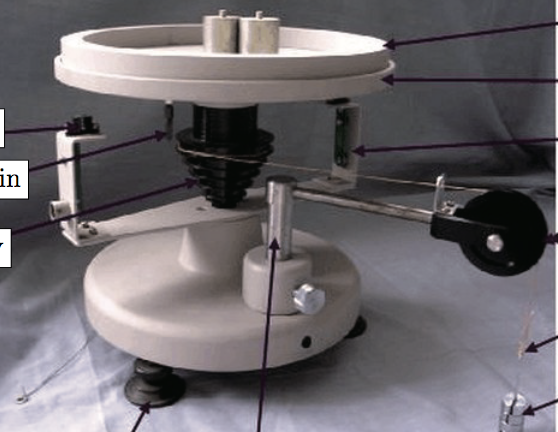
\includegraphics[width=10cm]{fig/app/turntable}
\end{figure}

Since the bearings of the turntable are not frictionless, there will be a
non-zero frictional torque $M_μ$ causing the turntable to decelerate with
angular acceleration $\beta_1$, so that the second law of dynamics for
rotational motion of the empty turntable reads $$   M_\mu = -I_1\beta_1  $$
\section{Procedure}

\section{Calculations and Results}

\section{Measurement Uncertianty Analysis}

\section{Conclusions and Discussion}

% data sheet

\end{document}